
\documentclass[a4paper,12pt]{article}

\usepackage[a4paper, total={6in, 8in}, left=30mm]{geometry}
\usepackage{pdfpages}

\usepackage{cmap}
\usepackage{caption}
\usepackage[T2A]{fontenc}
\usepackage[utf8]{inputenc}
\usepackage[english,russian]{babel}
\usepackage{fancyhdr}
\usepackage{hyperref}
\usepackage{amsmath}
\usepackage{graphicx}
\usepackage[document]{ragged2e}

\providecommand{\tightlist}{%
  \setlength{\itemsep}{0pt}\setlength{\parskip}{0pt}}

\hypersetup{
  pdfborderstyle={/S/U/W 1}
}

\graphicspath{./}

\pagestyle{fancy}
\fancyhf{}
\lhead{Антон Завьялов, ПИ-72}
\rhead{\textbf{Лабораторная №5}}
\cfoot{\thepage}

\makeatletter
\def\@seccntformat#1{%
  \expandafter\ifx\csname c@#1\endcsname\c@section\else
  \csname the#1\endcsname\quad
  \fi}
\makeatother

\begin{document}
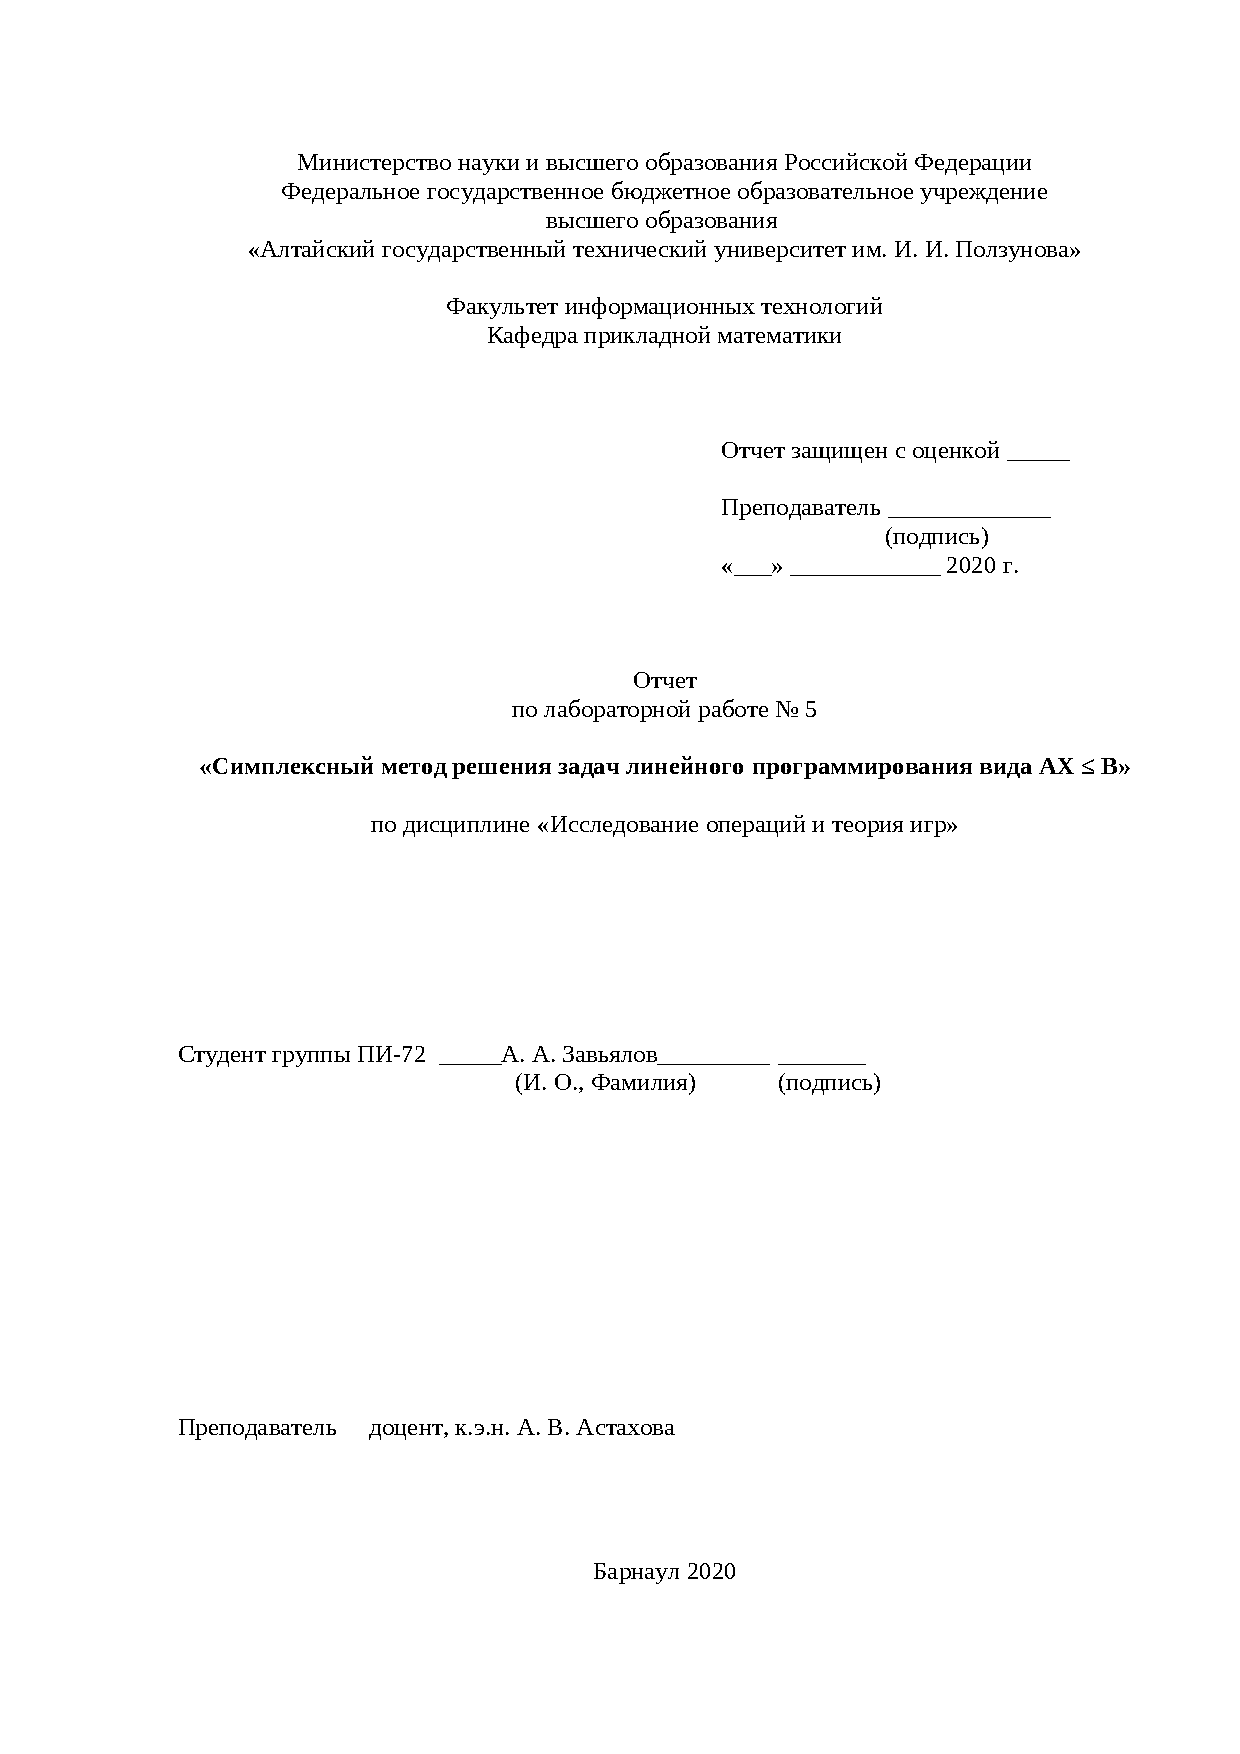
\includepdf[pages={1}]{title.pdf}

\section{\normalsize{Задание на лабораторную работу}}
\begin{flushleft}
\justify
\begin{enumerate}
\item
  Выбрать тестовый пример ЗЛП вида \textbf{AX $\le$ B} для освоения алгоритма симплекс метода.
\item
  Получить решение выбранной ЗЛП симплекс-методом с использованием аналитических преобразований, обосновав их правомерность. Записать ответ задачи.
\item
  Решить вручную данную задачу с использованием табличного симплекс метода. Оформить все симплекс-таблицы, обосновав полученные табличные результаты аналитическими преобразованиями, выполненными в п.3 данного задания. Записать ответ задачи.
\item 
  Проверить полученное решение с использованием выбранного инструментального средства в виде табличного процессора.
\end{enumerate}
\end{flushleft}

\pagebreak

\section{\normalsize{Выполнение работы}}
\begin{flushleft}
\justify
\begin{enumerate}
  \item Выбрана следующая задача:
    \begin{equation*}
      F = 2x_1 + 3x_2 - x_4 \rightarrow max
    \end{equation*}
    \begin{equation*}
      \begin{cases}
        2x_1 - x_2 - 2x_4 + x_5 \le 16 \\
        3x_1 + 2x_2 + x_3 - 3x_4 \le 18 \\
        -x_1 + 3x_2 + 4x_4 + x_6 \le 24
      \end{cases}
    \end{equation*}
    \begin{equation*}
      x_i \ge 0, i = 1, ..., 6
    \end{equation*}
  \item \textbf{Решение с использованием аналитических преобразований}\newline
    Через $x_0$ обозначим значение целевой функции и введём свободные переменные:
    \begin{equation*}
      \begin{cases}
        x_0 - 2x_1 - 3x_2 + x_4 = 0 & (0)\\
        2x_1 - x_2 - 2x_4 + x_5 + x_7 = 16 & (1) \\
        3x_1 + 2_x2 + x_3 - 3x_4 + x_8 = 18 & (2) \\
        -x_1 + 3x_2 + 4x_4 + x_6 + x_9 = 24 & (3)
      \end{cases}
    \end{equation*}
    Исходное базисное решение: $x_0 = 0, x_7 = 16, x_8 = 18, x_9 = 24$. В таком случае $x_0, x_7, x_8, x_9$ - базисные переменные, остальные переменные небазисные.

    В соответствии с критерием I, в базис следует ввести переменную $x_2$.

    Отношения чисел, стоящих в правых частях, к соответствующим коэффициентам при новой базисной переменной $x_2$: $~-16 (1),~9 (2),~8 (3)$. В соответствии с критерием II, выбирается наименьшее положительное отношение --- в нашем случае, 8, соответствующее уравнению №3. Из базиса выводится $x_9$.

    Система после замены базиса:
    \begin{equation*}
      \begin{cases}
        x_0 - 3x_1 + 5x_4 + x_6 + x_9 = 24 & (0)\\
        \frac{5}{3}x_1 - \frac{2}{3}x_4 + x_5 + \frac{1}{3}x_6 + \frac{1}{3}x_9 + x_7 = 24 & (1) \\
        \frac{11}{3}x_1 + x_3 - \frac{17}{3}x_4 - \frac{2}{3}x_6 - \frac{2}{3}x_9 + x_8 = 2 & (2) \\
        -\frac{1}{3}x_1 + x_2 + \frac{4}{3}x_4 + \frac{x_6}{3} + \frac{x_9}{3} = 8 & (3)  
      \end{cases}
    \end{equation*}

    По критерию I, т.к. в (0) есть отрицательный коэффициент при $x_1$, выбираем $x_1$ как новую базисную переменную.

    Отношения чисел, стоящих в правых частях, к соответствующим коэффициентам при новой базисной переменной $x_1$: $\frac{72}{5} (1),~\frac{6}{11}(2),~-24(3)$. В соответствии с критерием II, выбирается $\frac{6}{11}$, соотв. уравнению (2), поэтому из базиса выводится $x_8$.

    Система после замены базиса:
    \begin{equation*}
      \begin{cases}
        x_0 + \frac{9}{11}x_3 + \frac{4}{11}x_4 + \frac{5}{11}x_6 + \frac{5}{11}x_9 + \frac{9}{11}x_8 = \frac{282}{11} & (0) \\
        -\frac{5}{11}x_3 + \frac{21}{11}x_4 + x_5 + \frac{7}{11}x_6 + \frac{7}{11}x_9 - \frac{5}{11}x_8 + x_7 = \frac{254}{11} & (1) \\
        x_1 + \frac{3}{11}x_3 -\frac{17}{11}x_4 -\frac{2}{11}x_6 -\frac{2}{11}x_9 + \frac{3}{11}x_8 = \frac{6}{11} & (2) \\
        x_2 + \frac{1}{11}x_3 + \frac{9}{11}x_4 + \frac{3}{11}x_6 + \frac{3}{11}x_9 + \frac{1}{11}x_8 = \frac{90}{11} & (3)
      \end{cases}
    \end{equation*}

    В строке (0) все коэффициенты положительные, оптимальное решение получено:
    \begin{equation*}
      \begin{split}
        x_0 = \frac{282}{11}, \\
        x_7 = \frac{254}{11}, \\
        x_1 = \frac{6}{11}, \\
        x_2 = \frac{90}{11}.
      \end{split}
    \end{equation*}
    \begin{equation*}
      F_{max} = F(x_1 = \frac{6}{11}, x_2 = \frac{90}{11}, x_4 = 0) = \frac{282}{11}.
    \end{equation*}
    \textbf{Ответ:} $x_0 = \frac{282}{11}, x_7 = \frac{254}{11}, x_1 = \frac{6}{11}, x_2 = \frac{90}{11}, F_{max} = \frac{282}{11}.$
  \item \textbf{Решение задачи табличным методом}
    \begin{equation*}
      \begin{cases}
        x_0 - 2x_1 - 3x_2 + x_4 = 0 & (0)\\
        2x_1 - x_2 - 2x_4 + x_5 + x_7 = 16 & (1) \\
        3x_1 + 2_x2 + x_3 - 3x_4 + x_8 = 18 & (2) \\
        -x_1 + 3x_2 + 4x_4 + x_6 + x_9 = 24 & (3)
      \end{cases}
    \end{equation*}

    \begin{table}[h]
      \begin{center}
      \begin{tabular}{ |c|c|c|c|c|c|c|c| }
        \hline
        & св. & $x_1$ & $x_2$ & $x_3$ & $x_4$ & $x_5$ & $x_6$ \\
        \hline
        $x_7$ & 16 & 2 & -1 & 0 & -2 & 1 & 0 \\
        \hline
        $x_8$ & 18 & 3 & 2 & 1 & -3 & 0 & 0 \\
        \hline
        $x_9$ & 24 & -1 & 3 & 0 & 4 & 0 & 1 \\
        \hline
        $x_0$ & 0 & -2 & -3 & 0 & 1 & 0 & 0 \\
        \hline
      \end{tabular}
      \end{center}
      \caption{}
    \end{table}
    План не оптимален, т.к. есть отрицательные элементы на пересечении $x_0$ и небазисных переменных. $x_2$ заносится в базис, т.к. $x_0x_2$ - наибольшее по модулю число в строке. Соотношения $\frac{\textup{св.}}{x_2}$ построчно: $-1 (x_7),~9 (x_8),~8(x_9)$. Минимальное по модулю --- 8 $\implies x_2 \leftrightarrow x_9$. Строим новую таблицу:
    \newline
    \begin{table}[h]
      \begin{center}
        \begin{tabular}{ |c|c|c|c|c|c|c|c| }
          \hline
          & св. & $x_1$ & $x_9$ & $x_3$ & $x_4$ & $x_5$ & $x_6$ \\
          \hline
          $x_7$ & 24 & $\frac{5}{3}$ & $\frac{1}{3}$ & 0 & -$\frac{2}{3}$ & 1 & $\frac{1}{3}$ \\
          \hline
          $x_8$ & 2 & $\frac{11}{3}$ & -$\frac{2}{3}$ & 1 & -$\frac{17}{3}$ & 0 & -$\frac{2}{3}$ \\
          \hline
          $x_2$ & 8 & -$\frac{1}{3}$ & $\frac{1}{3}$ & 0 & $\frac{4}{3}$ & 0 & $\frac{1}{3}$ \\
          \hline
          $x_0$ & 24 & -3 & 1 & 0 & 5 & 0 & 1 \\
          \hline
        \end{tabular}
      \end{center}
      \caption{}
      \label{table:t_2}
    \end{table}

    План для таблицы \ref{table:t_2} не оптимален, т.к. $x_0x_1 = -3 < 0$. В базис заносится $x_1$. Соотношения $\frac{\textup{св.}}{x_1}$ построчно: $\frac{72}{5} (x_7),~\frac{6}{11} (x_8),~-24(x_9)$. Минимальное по модулю --- $\frac{6}{11} \implies x_1 \leftrightarrow x_8$. Строим новую таблицу:
    \begin{table}[h]
      \begin{center}
      \begin{tabular}{ |c|c|c|c|c|c|c|c| }
        \hline
        & св. & $x_8$ & $x_9$ & $x_3$ & $x_4$ & $x_5$ & $x_6$ \\
        \hline
        $x_7$ & $\frac{254}{11}$ & -$\frac{5}{11}$ & $\frac{7}{11}$ & -$\frac{5}{11}$ & $\frac{21}{11}$ & 1 & $\frac{7}{11}$ \\
        \hline
        $x_1$ & $\frac{6}{11}$ & $\frac{3}{11}$ & -$\frac{2}{11}$ & $\frac{3}{11}$ & -$\frac{17}{11}$ & 0 & -$\frac{22}{11}$ \\
        \hline
        $x_2$ & $\frac{90}{11}$ & $\frac{1}{11}$ & $\frac{3}{11}$ & $\frac{1}{11}$ & $\frac{9}{11}$ & 0 & $\frac{3}{11}$ \\
        \hline
        $x_0$ & $\frac{282}{11}$ & $\frac{9}{11}$ & $\frac{5}{11}$ & $\frac{9}{11}$ & $\frac{4}{11}$ & 0 & $\frac{5}{11}$ \\
        \hline
      \end{tabular}
      \end{center}
      \caption{}
    \end{table}

    Т.к. в $x_0$ отсутствуют отрицательные элементы, план оптимален.

    \textbf{Ответ:} $x_0 = \frac{282}{11}, x_7 = \frac{254}{11}, x_1 = \frac{6}{11}, x_2 = \frac{90}{11}, F_{max} = x_0 = \frac{282}{11}.$
  \item \textbf{Проверка решения с использованием табличного процессора}
  
    Использовался табличный процессор \textit{LibreOffice Calc}.
    \begin{figure}[h]
      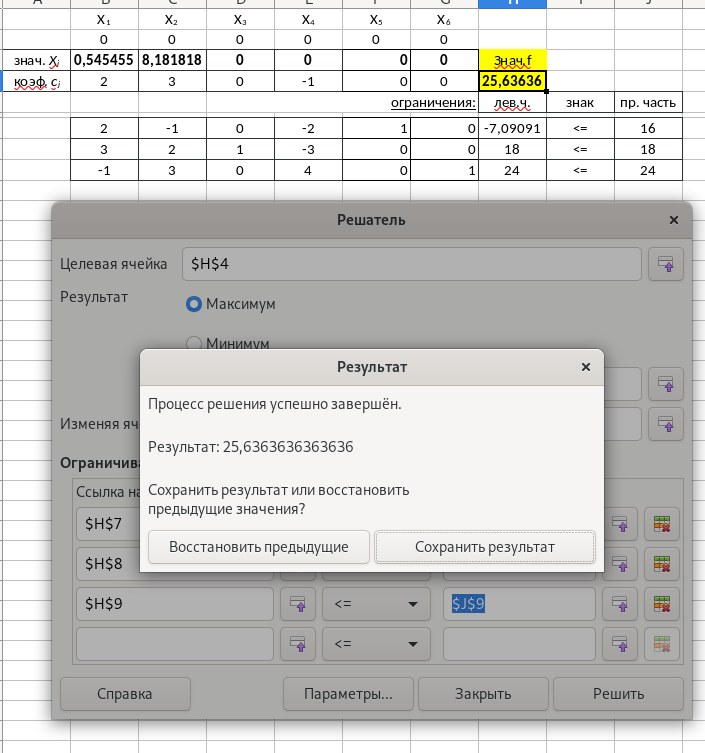
\includegraphics[width=15cm,height=16cm]{calc.png}      
    \end{figure}
\end{enumerate}
\end{flushleft}

\end{document}
